% !TEX root = task-3-16-5.tex
% Editable task bank. Append new BankTask blocks at the end of the document.
\documentclass[12pt,a4paper]{article}
\usepackage{physics-textbook}
\usepackage{graphicx,needspace}
\usetikzlibrary{decorations.pathmorphing}
\newif\ifShowSolutions
\ifdefined\TutorEdition
  \ShowSolutionstrue
\else
  \ShowSolutionsfalse % Change to \ShowSolutionstrue to display solutions.
\fi
\newcounter{banktask}
\newsavebox{\BankTaskBox}
\newcommand{\BankTaskContent}[3]{%
  \noindent\textbf{\thebanktask.}\quad #2\par
  \ifShowSolutions
    \Needspace{50mm}% Keep the solution heading with its opening text or diagram.
    #3\par
    \ifdefined\TutorEdition
      \ifcsname TutorSource#1\endcsname
        \nopagebreak\smallskip{\small\csname TutorSource#1\endcsname\par}%
      \fi
    \fi
  \fi
}
\newcommand{\BankTask}[3]{%
  \refstepcounter{banktask}\par\medskip
  \sbox{\BankTaskBox}{\begin{minipage}{\linewidth}%
    \BankTaskContent{#1}{#2}{#3}\end{minipage}}%
  \ifdim\dimexpr\ht\BankTaskBox+\dp\BankTaskBox\relax>\dimexpr\textheight-20mm\relax
    \Needspace{35mm}\BankTaskContent{#1}{#2}{#3}%
  \else
    \Needspace{\dimexpr\ht\BankTaskBox+\dp\BankTaskBox\relax}%
    \noindent\usebox{\BankTaskBox}\par
  \fi
  \medskip
}
\begin{document}
\BookSubsection{3.16.5}{p–n-переход}


% Source 25381: https://phys-ege.sdamgia.ru/problem?id=25381
\BankTask{25381}{
\begin{center}\begin{tikzpicture}[>=stealth,line width=.6pt]

\draw(0,1)--(0,1.91) (0,2.29)--(0,2.75)--(4.51,2.75)--(4.51,2.3) (4.51,1.92)--(4.51,1.0)
 (4.51,.58)--(4.51,-.14)--(0,-.14)--(0,.58)
 (1.65,2.75)--(1.65,2.29) (1.65,1.49)--(1.65,1.25) (1.65,1.11)--(1.65,.53)
 (2.91,2.75)--(2.91,1.25) (2.91,1.11)--(2.91,.53);
\fill(1.65,.53)circle(.042) (2.91,.53)circle(.042) (2.28,.24)circle(.042);
\draw (2.28,-.14)--(2.28,.24);
\node[left]at(1.65,.45){$1$};\node[right]at(2.91,.45){$2$};
\draw(2.28,.24)--(1.65,.53);\begin{scope}[shift={(0,2.1)},rotate=-90]\draw(-.2,-.16)--(-.2,.16)--(.18,0)--cycle (.18,-.18)--(.18,.18);\end{scope}\node[left] at (0,2.3000000000000003) {$\text{Д1}$};\begin{scope}[shift={(4.51,2.11)},rotate=90]\draw(-.2,-.16)--(-.2,.16)--(.18,0)--cycle (.18,-.18)--(.18,.18);\end{scope}\node[right] at (4.51,2.31) {$\text{Д2}$};\begin{scope}[shift={(0,0.79)}]\draw(0,0)circle(.21) (-.14,-.14)--(.14,.14) (-.14,.14)--(.14,-.14);\node[left]at(-.23,0){Л1};\end{scope}\begin{scope}[shift={(4.51,0.79)}]\draw(0,0)circle(.21) (-.14,-.14)--(.14,.14) (-.14,.14)--(.14,-.14);\node[left]at(-.23,0){};\end{scope}\node[right]at(4.72,.79){Л2};\begin{scope}[shift={(1.65,1.89)},rotate=90]\draw[fill=orange!35] (-.4,-.13) rectangle (.4,.13);\end{scope}\node[left] at (1.65,1.89) {$R$};\begin{scope}[shift={(1.65,1.18)},rotate=-90]\draw(-.07,-.21)--(-.07,.21) (.07,-.11)--(.07,.11);\end{scope}\node[above right] at (1.77,1.18) {$$};\begin{scope}[shift={(2.91,1.18)},rotate=90]\draw(-.07,-.21)--(-.07,.21) (.07,-.11)--(.07,.11);\end{scope}\node[above right] at (3.0300000000000002,1.18) {$$};\node[left]at(1.46,1.18){$\mathcal E,r$};\node[right]at(3.09,1.18){$\mathcal E,r$};
\end{tikzpicture}\end{center}
На рисунке изображена схема электрической цепи, состоящей из двух одинаковых источников тока с ЭДС $\mathcal{E}$ и внутренним сопротивлением r, резистора сопротивлением R, двух одинаковых ламп Л1 и Л2, двух идеальных диодов Д1 и Д2 и ключа К. Опираясь на законы электродинамики, объясните, какие изменения произойдут в работе этой цепи, если перевести ключ К из положения $1$ в положение $2$. Сравните накал ламп в этих двух случаях.
}{
\smallskip\noindent\textbf{Решение}\par
При замыкании первого ключа ток не идет через правый источник тока. В этом случае цепь будет иметь вид, показанный на рис. $1$. Направление тока от плюса к минусу. При этом через диод Д1 ток идет в прямом направлении, а через диод Д2  — в обратном. Известно, что идеальный диод обладает малым сопротивлением при прохождении тока в прямом направлении и бесконечным сопротивлением при прохождении тока в обратном направлении. Тогда эквивалентная схема будет иметь вид, показанный на рис. $2$. 
При переводе ключа во второе положение, ток не будет идти через левый источник. Цепь будет иметь вид, показанный на рис. $3$. В этом случае ток через диод Д2 будет идти в прямом направлении, а через диод Д1  — в обратном. Тогда эквивалентная схема будет иметь вид, показанный на рис. $4$. 


\begin{center}\begin{tikzpicture}[>=stealth,line width=.6pt]

\draw(0,1)--(0,1.91) (0,2.29)--(0,2.75)--(4.51,2.75)--(4.51,2.3) (4.51,1.92)--(4.51,1.0)
 (4.51,.58)--(4.51,-.14)--(0,-.14)--(0,.58)
 (1.65,2.75)--(1.65,2.29) (1.65,1.49)--(1.65,1.25) (1.65,1.11)--(1.65,.53)
 (2.91,2.75)--(2.91,1.25) (2.91,1.11)--(2.91,.53);
\fill(1.65,.53)circle(.042) (2.91,.53)circle(.042) (2.28,.24)circle(.042);
\draw (2.28,-.14)--(2.28,.24);
\node[left]at(1.65,.45){$1$};\node[right]at(2.91,.45){$2$};
\draw(2.28,.24)--(1.65,.53);\draw[->](1.57,1.55)--(1.57,2.42);\draw[->](.85,2.57)--(.1,2.57);\draw[->](.18,1.7)--(.18,1.1);\draw[->](.66,.04)--(1.4,.04);\draw[->](3.3,2.57)--(4.37,2.57);\begin{scope}[shift={(0,2.1)},rotate=-90]\draw(-.2,-.16)--(-.2,.16)--(.18,0)--cycle (.18,-.18)--(.18,.18);\end{scope}\node[left] at (0,2.3000000000000003) {$\text{Д1}$};\begin{scope}[shift={(4.51,2.11)},rotate=90]\draw(-.2,-.16)--(-.2,.16)--(.18,0)--cycle (.18,-.18)--(.18,.18);\end{scope}\node[right] at (4.51,2.31) {$\text{Д2}$};\begin{scope}[shift={(0,0.79)}]\draw(0,0)circle(.21) (-.14,-.14)--(.14,.14) (-.14,.14)--(.14,-.14);\node[left]at(-.23,0){Л1};\end{scope}\begin{scope}[shift={(4.51,0.79)}]\draw(0,0)circle(.21) (-.14,-.14)--(.14,.14) (-.14,.14)--(.14,-.14);\node[left]at(-.23,0){};\end{scope}\node[right]at(4.72,.79){Л2};\begin{scope}[shift={(1.65,1.89)},rotate=90]\draw[fill=orange!35] (-.4,-.13) rectangle (.4,.13);\end{scope}\node[left] at (1.65,1.89) {$R$};\begin{scope}[shift={(1.65,1.18)},rotate=-90]\draw(-.07,-.21)--(-.07,.21) (.07,-.11)--(.07,.11);\end{scope}\node[above right] at (1.77,1.18) {$$};\begin{scope}[shift={(2.91,1.18)},rotate=90]\draw(-.07,-.21)--(-.07,.21) (.07,-.11)--(.07,.11);\end{scope}\node[above right] at (3.0300000000000002,1.18) {$$};\node[left]at(1.46,1.18){$\mathcal E,r$};\node[right]at(3.09,1.18){$\mathcal E,r$};
\end{tikzpicture}\end{center}

Рис. $1$ 


\begin{center}\begin{tikzpicture}[>=stealth,line width=.6pt]
\draw(0,1.02)--(0,2.4)--(2.61,2.4)--(2.61,1.86) (2.61,1.06)--(2.61,.74) (2.61,.6)--(2.61,-.18)--(0,-.18)--(0,.6);\begin{scope}[shift={(0,0.81)}]\draw(0,0)circle(.21) (-.14,-.14)--(.14,.14) (-.14,.14)--(.14,-.14);\node[left]at(-.23,0){Л1};\end{scope}\begin{scope}[shift={(2.61,1.46)},rotate=90]\draw[fill=orange!35] (-.4,-.13) rectangle (.4,.13);\end{scope}\node[left] at (2.61,1.46) {$R$};\begin{scope}[shift={(2.61,0.67)},rotate=-90]\draw(-.07,-.21)--(-.07,.21) (.07,-.11)--(.07,.11);\end{scope}\node[above right] at (2.73,0.67) {$\mathcal E,r$};
\end{tikzpicture}\end{center}

Рис. $2$ 


\begin{center}\begin{tikzpicture}[>=stealth,line width=.6pt]

\draw(0,1)--(0,1.91) (0,2.29)--(0,2.75)--(4.51,2.75)--(4.51,2.3) (4.51,1.92)--(4.51,1.0)
 (4.51,.58)--(4.51,-.14)--(0,-.14)--(0,.58)
 (1.65,2.75)--(1.65,2.29) (1.65,1.49)--(1.65,1.25) (1.65,1.11)--(1.65,.53)
 (2.91,2.75)--(2.91,1.25) (2.91,1.11)--(2.91,.53);
\fill(1.65,.53)circle(.042) (2.91,.53)circle(.042) (2.28,.24)circle(.042);
\draw (2.28,-.14)--(2.28,.24);
\node[left]at(1.65,.45){$1$};\node[right]at(2.91,.45){$2$};
\draw(2.28,.24)--(2.91,.53);\draw[->](3.8,2.57)--(3.2,2.57);\draw[->](3.08,1.0)--(3.08,.27);\draw[->](4.36,1.24)--(4.36,1.86);\draw[->](2.15,.04)--(1.5,.04);\draw[->](.16,1.22)--(.16,1.79);\begin{scope}[shift={(0,2.1)},rotate=-90]\draw(-.2,-.16)--(-.2,.16)--(.18,0)--cycle (.18,-.18)--(.18,.18);\end{scope}\node[left] at (0,2.3000000000000003) {$\text{Д1}$};\begin{scope}[shift={(4.51,2.11)},rotate=90]\draw(-.2,-.16)--(-.2,.16)--(.18,0)--cycle (.18,-.18)--(.18,.18);\end{scope}\node[right] at (4.51,2.31) {$\text{Д2}$};\begin{scope}[shift={(0,0.79)}]\draw(0,0)circle(.21) (-.14,-.14)--(.14,.14) (-.14,.14)--(.14,-.14);\node[left]at(-.23,0){Л1};\end{scope}\begin{scope}[shift={(4.51,0.79)}]\draw(0,0)circle(.21) (-.14,-.14)--(.14,.14) (-.14,.14)--(.14,-.14);\node[left]at(-.23,0){};\end{scope}\node[right]at(4.72,.79){Л2};\begin{scope}[shift={(1.65,1.89)},rotate=90]\draw[fill=orange!35] (-.4,-.13) rectangle (.4,.13);\end{scope}\node[left] at (1.65,1.89) {$R$};\begin{scope}[shift={(1.65,1.18)},rotate=-90]\draw(-.07,-.21)--(-.07,.21) (.07,-.11)--(.07,.11);\end{scope}\node[above right] at (1.77,1.18) {$$};\begin{scope}[shift={(2.91,1.18)},rotate=90]\draw(-.07,-.21)--(-.07,.21) (.07,-.11)--(.07,.11);\end{scope}\node[above right] at (3.0300000000000002,1.18) {$$};\node[left]at(1.46,1.18){$\mathcal E,r$};\node[right]at(3.09,1.18){$\mathcal E,r$};
\end{tikzpicture}\end{center}

Рис. $3$ 


\begin{center}\begin{tikzpicture}[>=stealth,line width=.6pt]
\draw(0,1.04)--(0,2.37)--(2.61,2.37)--(2.61,1.18) (2.61,.76)--(2.61,-.18)--(0,-.18)--(0,.9);\begin{scope}[shift={(2.61,0.97)}]\draw(0,0)circle(.21) (-.14,-.14)--(.14,.14) (-.14,.14)--(.14,-.14);\node[left]at(-.23,0){Л2};\end{scope}\begin{scope}[shift={(0,0.97)},rotate=90]\draw(-.07,-.21)--(-.07,.21) (.07,-.11)--(.07,.11);\end{scope}\node[above right] at (0.12,0.97) {$$};\node[left]at(-.24,.97){$\mathcal E,r$};
\end{tikzpicture}\end{center}

Рис. $4$ 

В первом случае в цепи лампа Л1 и резистор соединены последовательно. Их общее сопротивление равно $R + R_{\,\text{л}}.$ По закону Ома для полной цепи, сила тока $I_1= \frac{\mathcal{E}}{R + R_{\,\text{л}} + r} .$
Во втором случае в цепи будет только лампа Л2. По закону Ома для полной цепи сила тока $I_2= \frac{\mathcal{E}}{R_{\,\text{л}} + r} .$ Очевидно, что сопротивление уменьшилось, а сила тока увеличилась. Мощность тока в первом случае:

\[P_1=I_1 ^2 R_{\,\text{л}}= \frac{\mathcal E^2 R_{\text{л}}}{(R+R_{\text{л}}+r)^2} ,\]

во втором случае:

\[P_2=I_2 ^2 R_{\,\text{л}}= \frac{\mathcal E^2 R_{\text{л}}}{(R_{\text{л}}+r)^2} .\]

Из приведенных формул видно, что мощность тока увеличилась, следовательно, при переводе ключа из положения $1$ в положение $2$ накал одной из ламп увеличится, а другая лампа гореть не будет.

Ответ: накал горящей лампы увеличится.
}

% Source 38951: https://phys-ege.sdamgia.ru/problem?id=38951
\BankTask{38951}{
Три одинаковых резистора и два одинаковых идеальных диода включены в электрическую цепь, показанную на рисунке, и подключены к аккумулятору в точках В и С. Показания амперметра равны $2\,\text{А}$. Определите силу тока через амперметр при смене полярности подключения аккумулятора. Нарисуйте эквивалентные электрические схемы для двух случаев подключения аккумулятора. Опираясь на законы электродинамики, поясните свой ответ. Сопротивлением амперметра и внутренним сопротивлением аккумулятора пренебречь.
\begin{center}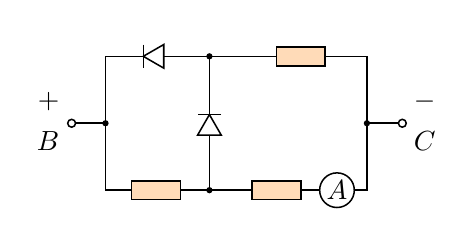
\begin{tikzpicture}[>=stealth,line width=.55pt]\draw(.5,.85)--(.88,.85) (.88,0)--(.88,1.7)--(4.2,1.7)--(4.2,0)--(.88,0) (4.2,.85)--(4.6,.85) (2.2,0)--(2.2,1.7);\fill(.88,.85)circle(.04) (4.2,.85)circle(.04) (2.2,0)circle(.04) (2.2,1.7)circle(.04);\draw(.45,.85)circle(.05) (4.65,.85)circle(.05);\node[left]at(.42,1.13){$+$};\node[left]at(.42,.63){$B$};\node[right]at(4.67,1.13){$-$};\node[right]at(4.67,.63){$C$};\begin{scope}[shift={(1.47,1.7)},rotate=180]\draw[fill=white](-.15,-.15)--(.11,0)--(-.15,.15)--cycle;\draw(.11,-.15)--(.11,.15);\end{scope}\begin{scope}[shift={(2.2,0.85)},rotate=90]\draw[fill=white](-.15,-.15)--(.11,0)--(-.15,.15)--cycle;\draw(.11,-.15)--(.11,.15);\end{scope}\draw[fill=orange!28](3.05,1.58)rectangle(3.67,1.8199999999999998);\node[above]at(3.36,1.8199999999999998){$$};\draw[fill=orange!28](1.21,-0.12)rectangle(1.83,0.12);\node[above]at(1.52,0.12){$$};\draw[fill=orange!28](2.7399999999999998,-0.12)rectangle(3.36,0.12);\node[above]at(3.05,0.12){$$};\draw[fill=white](3.82,0)circle(.22)node{$A$};\end{tikzpicture}\end{center}
}{
\smallskip\noindent\textbf{Решение}\par
При первом подключении цепи к источнику постоянного напряжения ток через верхний диод не проходит, через второй диод  — проходит, при этом точки, между которыми он находится, имеют равные потенциалы. Тогда эквивалентная схема имеет вид, изображенный на рис. $1$. Так как при параллельном соединении резисторы имеют одинаковое сопротивление, а амперметр идеальный, то через обе ветки идет ток, равный $2\,\text{А}$, а в неразветвленном участке цепи сила тока $I=I_1 + I_2=4\,\text{А}.$ Учитывая законы последовательного и параллельного соединения проводников, находим общее сопротивление цепи:   $R_{\,\text{общ}}= \frac{3R}{2} .$ Так как внутренним сопротивлением аккумулятора можно пренебречь, то напряжение на его клеммах равно по закону Ома $U=IR_{\,\text{общ}}=4 \cdot \frac{3R}{2} =6R.$
При изменении полярности подключения источника напряжения ток пройдет через оба диода, поэтому ток через левый резистор не пойдет. В этом случае получаем эквивалентную схему, изображенную на рис. $2$.
В цепи имеется два резистора, соединенные параллельно. Поэтому общее сопротивление цепи станет равным $R'_{\,\text{общ}}= \frac{R}{2} ,$ а общая сила тока $I'= \frac{U}{R'_{\,\text{общ}}} =12\,\text{А}.$ Так как обе ветви параллельно соединенных участков имеют одинаковое сопротивление, то ток через резистор и амперметр будет равен $I_A= \frac{I'}{2} = \frac{12}{2} =6\,\text{А}.$

\begin{center}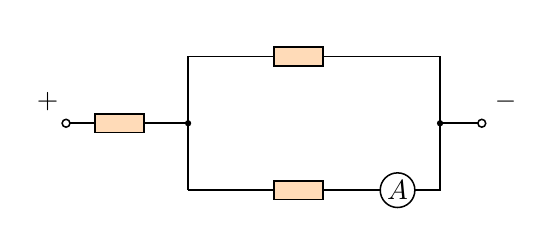
\begin{tikzpicture}[>=stealth,line width=.55pt]\draw(1,0)--(1,1.7)--(4.2,1.7)--(4.2,0)--(1,0);\fill(1,.85)circle(.04) (4.2,.85)circle(.04);\draw(4.2,.85)--(4.68,.85);\draw(4.73,.85)circle(.05);\draw(-.5,.85)--(1,.85);\draw(-.55,.85)circle(.05);\node[left]at(-.52,1.13){$+$};\node[right]at(4.77,1.13){$-$};\draw[fill=orange!28](-0.18,0.73)rectangle(0.44,0.97);\node[above]at(0.13,0.97){$$};\draw[fill=orange!28](2.09,1.58)rectangle(2.71,1.8199999999999998);\node[above]at(2.4,1.8199999999999998){$$};\draw[fill=orange!28](2.09,-0.12)rectangle(2.71,0.12);\node[above]at(2.4,0.12){$$};\draw[fill=white](3.66,0)circle(.22)node{$A$};\end{tikzpicture}\end{center}
Рис. $1$

\begin{center}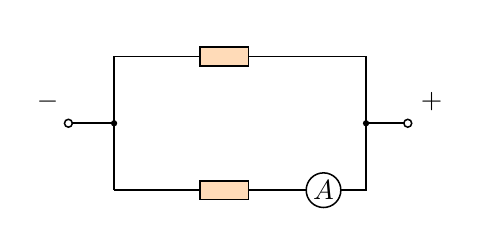
\begin{tikzpicture}[>=stealth,line width=.55pt]\draw(1,0)--(1,1.7)--(4.2,1.7)--(4.2,0)--(1,0);\fill(1,.85)circle(.04) (4.2,.85)circle(.04);\draw(4.2,.85)--(4.68,.85);\draw(4.73,.85)circle(.05);\draw(.47,.85)--(1,.85);\draw(.42,.85)circle(.05);\node[left]at(.42,1.13){$-$};\node[right]at(4.77,1.13){$+$};\draw[fill=orange!28](2.09,1.58)rectangle(2.71,1.8199999999999998);\node[above]at(2.4,1.8199999999999998){$$};\draw[fill=orange!28](2.09,-0.12)rectangle(2.71,0.12);\node[above]at(2.4,0.12){$$};\draw[fill=white](3.66,0)circle(.22)node{$A$};\end{tikzpicture}\end{center}
Рис. $2$

Ответ: сила тока через амперметр станет равной $6\,\text{А}$.
}

% Source 8554: https://phys-ege.sdamgia.ru/problem?id=8554
\BankTask{8554}{
\begin{center}\begin{tikzpicture}[>=stealth,line width=.55pt]\draw(0,2.1)--(-.55,1.95)--(-.55,.42)--(0,.19)--(.53,.42)--(.53,1.95)--(0,2.1);\draw(0,2.1)..controls(1.65,2.05)and(2.26,1.53)..(2.2,1.2)..controls(2.02,.55)and(1.96,.88)..(2.17,1.24)..controls(2.5,1.73)and(2.5,.98)..(2.24,.73)..controls(1.55,.27)and(.64,.19)..(0,.19);\foreach \x/\i in {-.55/1,.53/2}{\draw[fill=white](\x,1.59)circle(.19);\draw(\x-.13,1.46)--(\x+.13,1.72) (\x-.13,1.72)--(\x+.13,1.46);\node[left]at(\x-.19,1.57){$\i$};}\node[above]at(0,2.1){А};\node[below]at(0,.19){Б};\draw[->](.5,2.9)--(1.27,2.9);\draw[<-](.5,3.19)--(1.27,3.19);\draw(.98,3.05)--(1.16,3.33) (1.16,3.05)--(.98,3.33);\node[left]at(.35,3.02){$I$};\draw(.5,2.52)--(1.27,2.52);\draw[fill=cyan!25](2.9,.9)rectangle(3.55,1.48)node[pos=.5]{$N$};\draw[fill=red!25](3.55,.9)rectangle(4.2,1.48)node[pos=.5]{$S$};\draw[->,orange!85!black](4.08,.64)--(3.02,.64);\begin{scope}[shift={(-0.55,0.94)},rotate=-90]\draw[fill=white](-.15,-.15)--(.11,0)--(-.15,.15)--cycle;\draw(.11,-.15)--(.11,.15);\end{scope}\begin{scope}[shift={(0.53,0.94)},rotate=90]\draw[fill=white](-.15,-.15)--(.11,0)--(-.15,.15)--cycle;\draw(.11,-.15)--(.11,.15);\end{scope}\begin{scope}[shift={(0.97,2.52)},rotate=0]\draw[fill=white](-.15,-.15)--(.11,0)--(-.15,.15)--cycle;\draw(.11,-.15)--(.11,.15);\end{scope}\end{tikzpicture}\end{center}Электрическая цепь состоит из двух лампочек, двух диодов и витка провода, соединенных как показано на рисунке. (Диод пропускает ток только в одном направлении, как показано в верхней части рисунка.) Какая из лампочек загорится, если к витку приближать северный полюс магнита? Ответ объясните, указав, какие явления и закономерности Вы использовали при объяснении.
}{
\smallskip\noindent\textbf{Решение}\par
$1$.  Загорится лампочка $2$.
$2$.  При приближении магнита к витку будет меняться магнитный поток сквозь виток, и в витке возникнет индукционный ток. Согласно правилу Ленца магнитное поле этого тока должно препятствовать движению магнита, поэтому выходящие из витка линии индукции этого поля будут направлены в сторону магнита. Для создания такого поля, согласно правилу «буравчика», индукционный ток в цепи, содержащей виток, должен быть направлен по часовой стрелке (если смотреть слева), а в цепи ламп  — от Б к А. Ток такого направления пропускает только диод на участке цепи лампочки $2$, она и будет гореть.
}

% Source 41557: https://phys-ege.sdamgia.ru/problem?id=41557
\BankTask{41557}{
\begin{center}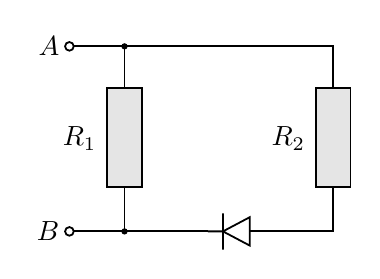
\begin{tikzpicture}[>=stealth,line width=.65pt]\draw (0,2.35)--(3.35,2.35)--(3.35,1.82) (3.35,.56)--(3.35,0)--(2.29,0) (1.76,0)--(0,0) (.7,2.35)--(.7,1.82) (.7,.56)--(.7,0);\draw[fill=gray!20](.48,.56)rectangle(.92,1.82) (3.13,.56)rectangle(3.57,1.82);\draw(2.29,0)--(2.29,.18)--(1.95,0)--(2.29,-.18)--cycle (1.95,.23)--(1.95,-.23) (1.95,0)--(1.76,0);\foreach \p in {(.7,0),(.7,2.35)}{\fill \p circle(.04);}\draw[fill=white](0,0)circle(.055) (0,2.35)circle(.055);\node[left]at(0,2.35){$A$};\node[left]at(0,0){$B$};\node[left]at(.47,1.18){$R_1$};\node[left]at(3.12,1.18){$R_2$};\end{tikzpicture}\end{center}

В цепи, изображённой на рисунке, сопротивление диода в прямом направлении пренебрежимо мало, а в обратном многократно превышает сопротивление резисторов. При подключении к точке A положительного, а к точке B  — отрицательного полюса батареи с ЭДС $6\,\text{В}$ и пренебрежимо малым внутренним сопротивлением потребляемая мощность (тепловая мощность, выделяемая во внешней цепи) равна $13$ Вт. При изменении полярности подключения батареи потребляемая мощность равна $9$ Вт.
Укажите для обоих случаев подключения батареи, протекает ли ток через диод и каждый из резисторов или нет, и определите сопротивления резисторов в этой цепи.
}{
\smallskip\noindent\textbf{Решение}\par
\begin{center}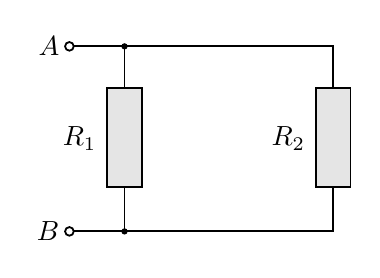
\begin{tikzpicture}[>=stealth,line width=.65pt]\draw (0,2.35)--(3.35,2.35)--(3.35,1.82) (3.35,.56)--(3.35,0)--(0,0) (.7,2.35)--(.7,1.82) (.7,.56)--(.7,0);\draw[fill=gray!20](.48,.56)rectangle(.92,1.82) (3.13,.56)rectangle(3.57,1.82);\foreach \p in {(.7,0),(.7,2.35)}{\fill \p circle(.04);}\draw[fill=white](0,0)circle(.055) (0,2.35)circle(.055);\node[left]at(0,2.35){$A$};\node[left]at(0,0){$B$};\node[left]at(.47,1.18){$R_1$};\node[left]at(3.12,1.18){$R_2$};\end{tikzpicture}\end{center}

 рис. а) 

Если подключить к точке А положительный полюс батареи, а к точке В  — отрицательный, то ток через диод идет. С учетом условия, что в прямом направлении его сопротивление пренебрежимо мало, получаем эквивалентную схему а), в которой два резистора соединены параллельно. Их общее сопротивление находится из формулы 

\[\frac{1}{R} = \frac{1}{R_1} + \frac{1}{R_2} .\]

С учетом, что внутреннее сопротивление батареи пренебрежимо мало, $U= \mathcal{E} ,$ потребляемая мощность равна

\[P_1= \frac{\mathcal{E} ^2}{R} .\]



\begin{center}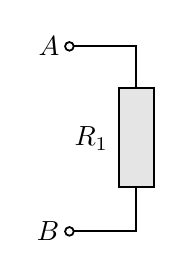
\begin{tikzpicture}[>=stealth,line width=.65pt]\draw (0,2.35)--(.85,2.35)--(.85,1.82) (.85,.56)--(.85,0)--(0,0);\draw[fill=gray!20](.63,.56)rectangle(1.07,1.82);\draw[fill=white](0,0)circle(.055) (0,2.35)circle(.055);\node[left]at(0,2.35){$A$};\node[left]at(0,0){$B$};\node[left]at(.62,1.18){$R_1$};\end{tikzpicture}\end{center}

 рис. б) 

 Если изменить полярность подключения, то ток через диод не пойдет, а, следовательно, не пройдет через резистор $R_{2}$. В этом случае эквивалентная схема будет иметь вид, представленный на рис. б). Мощность тока в этом случае будет равна

\[P_2= \frac{\mathcal{E} ^2}{R_1,}\]

откуда находим сопротивление первого резистора:

\[R_1= \frac{\mathcal{E} ^2}{P_2} = \frac{36}{9} =4\,\text{Ом}.\]

Тогда сопротивление второго резистора равно

\[R_2= \frac{\mathcal{E} ^2}{P_1 - P_2} = \frac{36}{13 - 9} =9\,\text{Ом}.\]

Ответ: $R_1=4\,\text{Ом}; R_2=9\,\text{Ом}.$
}

\end{document}
